\chapter{Frequency Modulated Continuous Wave Detection}

\section{FMCW Radar}
\label{sec:FMCWRadar}

The theory behind Frequency Modulated Continuous Wave (FMCW) detection will 
be explored in this section following the development of Brooker\cite{brooker2009}.
Booker's development focuses on FMCW radar, but the same theory applies to 
FMCW lidar by making the appropriate changes in the system hardware. For example, 
the antennae would be replaced with a telescope etc.   

\subsection{Basic Principles}

FMCW detection refers to a radar/lidar 
system in which a continuous wave of known frequency is modulated in amplitude,
transmitted, and the reflected signal is detected. A continuous wave radar in 
which a single microwave oscillator serves as both
the transmitter and local oscillator (LO) is, generally speaking, a homodyne radar.
Frequency modulated continuous waveform (FMCW) radar systems often leverage a 
homodyne architecture.

An FMCW radar uses a continuous wave signal which is modulated in amplitude 
over a range of frequencies creating a linear chirp. This chirped signal is 
radiated to the target and an echo 
returns after time $T_p$, which is the time it takes for the signal to reach the
target and reflected energy to return to the antennae. Figure~\ref{fig:doppShift}
illustrates a chirped signal, shown with a solid line, and the return signal delayed
by $T_p$, shown with a dashed line. In this figure $f_b$ refers to the difference in 
frequency of the two signals at a given time.  

\begin{figure}
	\begin{center}
		\begin{tikzpicture}[every text node part/.style={align=center}]
			\draw[thick,->] (1,1) -- (7,1) node[anchor=north] {Time};
			\draw[thick,->] (1,1) -- (1,5) node[anchor=south] {Freq};
			\draw (1,1) -- (5,5);
			\draw[dashed] (2.5,1) -- (6.5,5);
			\draw[dashed,<->] (4,2.6) -- (4,3.9) node[pos=0.5, anchor = east] {$f_b$};
			\draw[dashed,<->] (1,.8) -- (2.5,.8) node[pos=0.5, anchor = north] {$T_p$};
			\draw[dashed,<->] (1,0) -- (5,0) node[pos=0.5, anchor = north] {$T_b$};
		\end{tikzpicture}
		\caption{Transmit and Receive Doppler Shift}
		\label{fig:doppShift}
	\end{center}
\end{figure}

It is clear that the distance to the target can be calculated with $T_p$. In an FMCW system
$T_p$ is determined by measuring the beat frequency $f_b$. To do this a portion of the signal
produced by the LO is mixed with the returned echo producing $f_b$. A signal chirped in frequency
can be expressed as
\begin{equation}
\label{eq:chirpSig}
v_{fm}(t)=A_c cos[\omega_ct+\frac{A_b}{2} t^2].
\end{equation}
Where $A_b$ is a constant of proportionality between the change in frequency over the chirp or chirp slope, $\omega_b$,
and the chirp time; such that $\omega_b=A_bt$. The mixture of the transmitted and received signals can be 
expressed as
\begin{equation}
\label{eq:mixSig}
v_{fm}(t-T_p)v_{fm}(t)=A_c^2 cos[\omega_c t +\frac{A_b}{2}t^2]cos[\omega_c(t-T_p)+\frac{A_b}{2} (t-T_p)^2].
\end{equation}
This simplifies to 
\begin{equation}
\label{eq:mixSigOut}
v_{out}(t)=A_c^2 (cos[(2\omega_c-A_bT_p)t+A_bt^2+(\frac{A_b}{2}T_p^2-\omega_cT_p)]+cos[A_bT_pt+(\omega_cT_p-\frac{A_b}{2}T_p^2)]).
\end{equation}
It is desirable to isolate the second term in Eq~\ref{eq:mixSigOut} because it is the the beat signal. 
The first cosine term is an FM chirp at about twice the carrier frequency and is in most cases 
conveniently filtered out because it is above the cutoff frequency of the receiver components.
To obtain the $f_b$ from the beat signal the phase term is differentiated with time, 
\begin{equation}
\label{eq:phaseDiff}
f_b=\frac{1}{2\pi}\frac{d}{dt}[A_bT_bt+(\omega_cT_p-\frac{A_b}{2}T_p^2)],
\end{equation}
resulting in
\begin{equation}
\label{eq:fb}
f_b=(\frac{A_b}{2\pi})T_p.
\end{equation}

\subsection{FMCW Detection}
As discussed above, the most common way to obtain the beat frequency, $f_b$, is to 
take the product of the transmitted chirp signal and the received signal and filter 
to isolate the constant frequency beat. The Fast Fourier Transform (FFT) is the most
common method of spectral analysis employed in FMCW radar to measure $f_b$. 

Given a chirp duration, $T_b$(s), and assuming that $T_b$$\gg$$T_p$, the maximum resolution
of the beat frequency is 2/$T_b$(Hz). Figure \ref*{fig:doppShift} shows a chirp which meets 
that criterion. The resolution bandwidth of a signal, $\delta$$f_b$, is commonly defined 
between its 3 dB points. For the truncated chirp case  $\delta$$f_b$ coincides with a
region of width 1/$T_b$ centered on $f_b$, as shown in figure \ref{fig:trunkSpect}. 

\begin{figure}
	\begin{center}
		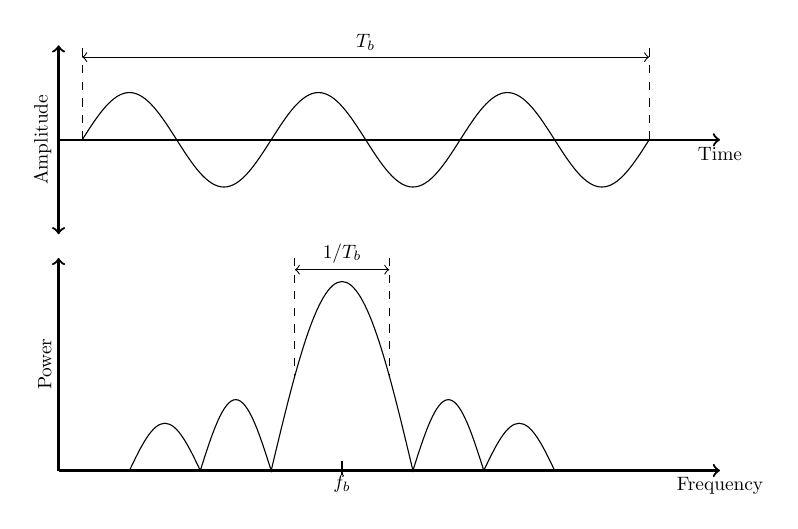
\begin{tikzpicture}[scale = .6,every text node part/.style={align=center}]
		\draw[thick,->] (1,8) -- (15,8) node[anchor=north,scale=0.7] {Time};
		\draw[thick,<->] (1,6) -- (1,10) node[pos = 0.5,above,scale=0.7,rotate=90] {Amplitude};
		\draw[thick,->] (1,1) -- (15,1) node[anchor=north,scale=0.7] {Frequency};
		\draw[thick,->] (1,1) -- (1,5.5) node[pos = 0.5,above,scale=0.7,rotate=90] {Power};
		\draw (2.5,1) sin (3.25,2) cos (4,1) sin (4.75,2.5) cos (5.5,1)  sin (7,5)  cos (8.5,1)
		sin (9.25,2.5) cos (10,1) sin (10.75,2) cos (11.5,1);  
		\draw (1.5,8) sin (2.5,9) cos (3.5,8) sin (4.5,7) cos (5.5,8) sin (6.5,9) cos (7.5,8)
		sin (8.5,7) cos (9.5,8) sin (10.5,9) cos (11.5,8) sin (12.5,7) cos (13.5,8);
		\draw[<->] (1.5,9.75) -- (13.5,9.75) node[pos = 0.5,anchor = south,scale=0.7] {$T_b$};
		\draw[dashed] (1.5,8) -- (1.5,10);
		\draw[dashed] (13.5,8) -- (13.5,10);
		\draw[<->] (6,5.25) -- (8,5.25) node[pos = 0.5,anchor = south,scale=0.7] {1/$T_b$};
		\draw[dashed] (6,5.5) -- (6,3);
		\draw[dashed] (8,5.5) -- (8,3);
		\draw (7,1.2) -- (7,.9) node[pos=0.5,below,scale=0.7] {$f_b$};
		\end{tikzpicture}
		\caption{Spectrum of the truncated sinusoidal signal output by an FMCW radar.}
		\label{fig:trunkSpect}
	\end{center}
\end{figure}

The chirp bandwidth is the total change in frequency for the chirp, $\Delta$$f$. Clearly
the slope of the chirp is the chirp bandwidth divided by the chirp time, $\Delta$$f$/$T_b$.
Eq \ref{eq:fb} can then be restated
\begin{equation}
	\label{eq:fb_alt}
	f_b=(\frac{A_b}{2\pi})T_p=\frac{\Delta f}{T_b}T_p.
\end{equation}
Intuitively $T_p$ is the round trip time from the antennae to the target and back
\begin{equation}
	\label{eq:roundTrip}
	T_p=2\frac{2R}{c},
\end{equation}
where c is the speed of light. The classical FMCW formula is obtained by substituting 
into eq \ref{eq:fb_alt}:
\begin{equation}
	\label{eq:classicFMCW}
	f_b=\frac{\Delta f}{T_b}\frac{2R}{c},
\end{equation}
relating the beat frequency to the range. Solving for range yields
\begin{equation}
\label{eq:FMCWrange}
R=\frac{T_bc}{2\Delta f}f_b.
\end{equation}

Eq \ref{eq:FMCWrange} relates range to beat frequency. The same equation can be used
to related range resolution $\delta$$f$ and chirp bandwidth:
\begin{equation}
	\label{eq:FMCWres}
	\delta R=\frac{T_bc}{2\Delta f}\delta f=\frac{c}{2\Delta f}.
\end{equation}
Where the frequency resolution $delta$$f$ is approximately equal to 1/$T_b$. 

\subsection{Doppler Effect in FMCW}
So far the development in this section has assumed a stationary radar and target. The 
case where the radar, the target, or both are moving will now be examined. The Doppler 
effect describes the change in observed and transmitted frequencies when the distance 
between the two is changing. The relationship between the transmitted frequency, $f_c$, 
and the received frequency, $f_r$ can be expressed
\begin{equation}
	\label{eq:dop1}
	f_r=\frac{c+v_t}{c+v_s}f_c.
\end{equation}
Where $v_t$ is the velocity of the target and $v_s$ is the velocity of the source. From
eq \ref{eq:dop1} it is simple to obtain an equation for the change in frequency, $\Delta$f
in relation to the difference in velocity of the source and target, $\Delta$$v$:
\begin{equation}
\label{eq:dop2}
\Delta f=\frac{\Delta v}{c}f_s.
\end{equation}
 
For the following development the radial velocity, $v_r$(m/s), will represent the velocity 
term causing the Doppler effect. Modifying eq \ref{eq:chirpSig} to incorporate the Doppler 
shift of the echo signal yields:
 
\begin{equation}
	\label{eq:chirpSigDop}
	v_{fm}(t-T_p)=A_c cos[\omega_c(t-T_p)+\frac{A_b}{2} (t-T_p)^2-\frac{2v_r}{c}\omega_c(t-T_p)].
\end{equation}
  
The new beat frequency then is the same as derived in eqs \ref{eq:fb} and \ref{eq:fb_alt} shifted
by the Doppler frequency, $f_d$:
\begin{equation}
	\label{eq:fbDop}
	f_b=\frac{2v_r}{c}f_c-\frac{A_b}{2\pi}T_p
	  =f_d-\frac{A_b}{2\pi}T_p.
\end{equation}

For a chirp with positive $A_b$, an up-chirp, the beat frequency will be the difference between 
the Doppler frequency $f_d$ and the beat frequency caused by the echo time or range frequency $f_r$. For a down-chirp, a negative
slope, the beat frequency will be the sum of the Doppler frequency and the range frequency. In many radar applications
it can be assumed that the Doppler frequency is lower than the range frequency leading to eqs \ref{eq:fbUp} and \ref{eq:fbDown}.
If $f_d$ > $f_b$, as is frequently the case in Lidar, the roles of $f_d$ and $f_b$ are reversed. 

\begin{equation}
\label{eq:fbUp}
f_{bUp}=f_b - f_d
\end{equation}

\begin{equation}
\label{eq:fbDown}
f_{bDown}=f_b + f_d
\end{equation}

By using a triangle waveform the sum and difference frequencies can be obtained to isolated range and velocity measurements. 
Fig \ref{fig:UpDownChirp} illustrates the Doppler effect on an FMCW waveform transmitting a triangle wave pattern.  
Expressions for $f_r$ and $f_d$ can be obtained by averaging and differencing eqs  \ref{eq:fbUp} and \ref{eq:fbDown}:
 \begin{equation}
 \label{eq:fr}
 f_r = \frac{f_{b(Up)}-f_{b(Down)}}{2},
 \end{equation}
 \begin{equation}
\label{eq:fd}
f_d = \frac{f_{b(Up)}+f_{b(Down)}}{2}.
\end{equation}
The sign of $f_d$ is determined by the direction of motion. If the range is getting smaller $f_d$ will be positive 
and if the range is getting larger $f_d$ will be negative. 

\begin{figure}
	\begin{center}
		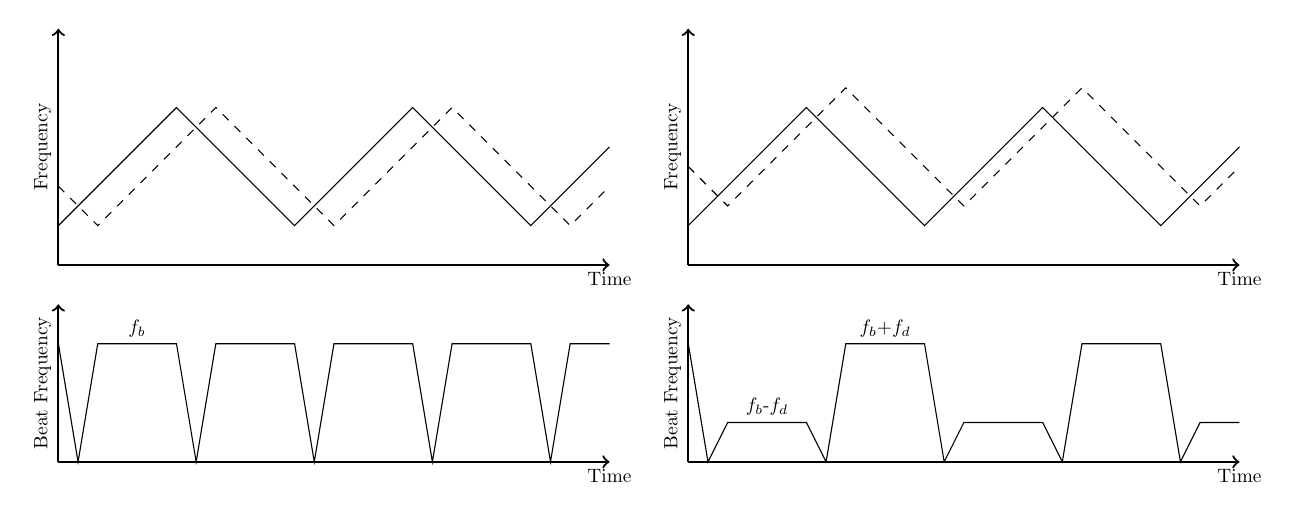
\begin{tikzpicture}[scale = .5,every text node part/.style={align=center}]
		%Left set of graphs
		\draw[thick,->] (1,6) -- (15,6) node[anchor=north,scale=0.7] {Time};
		\draw[thick,->] (1,6) -- (1,12) node[pos = 0.5,above,scale=0.7,rotate=90] {Frequency};
		\draw[thick,->] (1,1) -- (15,1) node[anchor=north,scale=0.7] {Time};
		\draw[thick,->] (1,1) -- (1,5) node[pos = 0.5,above,scale=0.7,rotate=90] {Beat Frequency};
		%transmit
		\draw (1,7) -- (4,10) -- (7,7) -- (10,10) -- (13,7) -- (15,9);
		\draw[dashed] (1,8) -- (2,7) -- (5,10) -- (8,7) -- (11,10) -- (14,7) -- (15,8);
		
		%beat
		\draw (1,4) -- (1.5,1) -- (2,4) -- (4,4) -- (4.5,1) -- (5,4) -- (7,4) -- (7.5,1) -- (8,4)
			  -- (10,4) -- (10.5,1) -- (11,4) -- (13,4) -- (13.5,1) -- (14,4) -- (15,4);
		\draw (2,4) -- (4,4) node[pos = 0.5,above,scale=0.7] {$f_b$};
		
		
		%Right set of graphs
		\draw[thick,->] (17,6) -- (31,6) node[anchor=north,scale=0.7] {Time};
		\draw[thick,->] (17,6) -- (17,12) node[pos = 0.5,above,scale=0.7,rotate=90] {Frequency};
		\draw[thick,->] (17,1) -- (31,1) node[anchor=north,scale=0.7] {Time};
		\draw[thick,->] (17,1) -- (17,5) node[pos = 0.5,above,scale=0.7,rotate=90] {Beat Frequency};
		%transmit
		\draw (17,7) -- (20,10) -- (23,7) -- (26,10) -- (29,7) -- (31,9);
		\draw[dashed] (17,8.5) -- (18,7.5) -- (21,10.5) -- (24,7.5) -- (27,10.5) -- (30,7.5) -- (31,8.5);
		
		%beat
		\draw (17,4) -- (17.5,1) -- (18,2) -- (20,2) -- (20.5,1) -- (21,4) -- (23,4) -- (23.5,1) -- (24,2)
		-- (26,2) -- (26.5,1) -- (27,4) -- (29,4) -- (29.5,1) -- (30,2) -- (31,2);
		
		\draw (18,2) -- (20,2) node[pos = 0.5,above,scale=0.7] {$f_b$-$f_d$};
		\draw (21,4) -- (23,4) node[pos = 0.5,above,scale=0.7] {$f_b$+$f_d$};
		
		\end{tikzpicture}
		\caption{Doppler Effect on FMCW radar.}
		\label{fig:UpDownChirp}
	\end{center}
\end{figure}

\section{FMCW Lidar Processing}
The two main differences between FMCW lidar and radar are the modulation frequencies and the wavelength of the 
radiation. One consequence of this is that the doppler frequency is usually higher than the beat frequency, 
leading to some minor modifications to the equations in section \ref{sec:FMCWRadar}. The most importantly the 
relationship between beat frequency of the up-chirp with the doppler frequency is better expressed as:

\begin{equation}
\label{eq:fbUpLaser}
f_{bUp}=f_d - f_b.
\end{equation}

In a practical FMCW lidar system it is common to add a period of constant frequency between up and down chirps in
the chirp process illustrated in figures \ref{fig:UpDownChirp}. Doing this gives a 
direct measurement of the Doppler frequency. This modified chirp process is shown in figure \ref{fig:UpDownFlatChirp}. 

\begin{figure}
	\begin{center}
		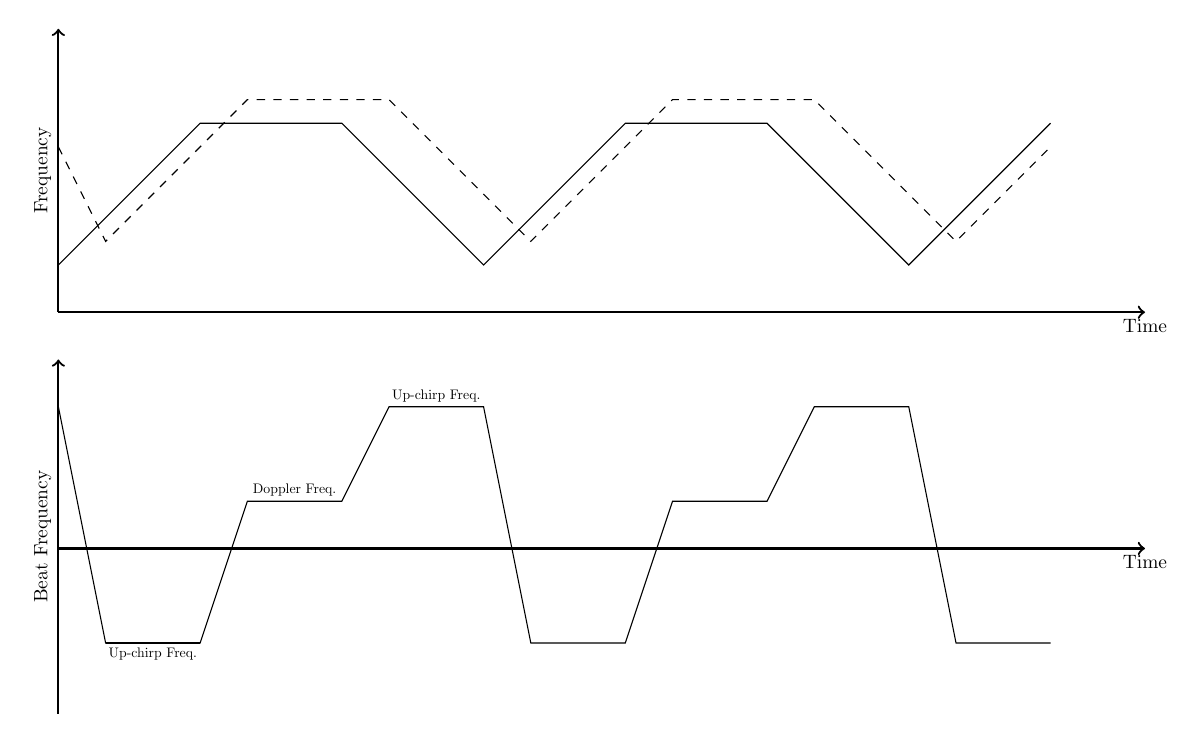
\begin{tikzpicture}[scale = .6,every text node part/.style={align=center}]
		\draw[thick,->] (1,6) -- (24,6) node[anchor=north,scale=0.7] {Time};
		\draw[thick,->] (1,6) -- (1,12) node[pos = 0.5,above,scale=0.7,rotate=90] {Frequency};
		\draw[thick,->] (1,1) -- (24,1) node[anchor=north,scale=0.7] {Time};
		\draw[thick,->] (1,-2.5) -- (1,5) node[pos = 0.5,above,scale=0.7,rotate=90] {Beat Frequency};
		%transmit
		\draw (1,7) -- (4,10) -- (7,10) -- (10,7) -- (13,10) -- (16,10) -- (19,7) -- (22,10);
		\draw[dashed] (1,9.5)-- (2,7.5) -- (5,10.5) -- (8,10.5) -- (11,7.5) -- (14,10.5) -- (17,10.5) -- (20,7.5) -- (22,9.5);;
		
		%beat
		\draw (1,4) -- (2,-1) -- (4,-1)  -- (5,2) -- (7,2) -- (8,4) -- (10,4) -- (11,-1) -- (13,-1)
		-- (14,2) -- (16,2) -- (17,4) -- (19,4) -- (20,-1) -- (22,-1);
		
		\draw (2,-1) -- (4,-1) node[pos = 0.5,below,scale=0.5] {Up-chirp Freq.};
		\draw (5,2) -- (7,2) node[pos = 0.5,above,scale=0.5] {Doppler Freq.};
		\draw (8,4) -- (10,4) node[pos = 0.5,above,scale=0.5] {Up-chirp Freq.};
		
		\end{tikzpicture}
		\caption{Doppler Effect on FMCW lidar with up-chirp, steady, and down-chirp sections.}
		\label{fig:UpDownFlatChirp}
	\end{center}
\end{figure}

From the process process illustrated in figure \ref{fig:UpDownFlatChirp} the system obtains three measured frequencies:
$f_{b(Up)}$ the up-chirp frequency, $f_d$ the Doppler frequency, and $f_{b(Down)}$ the down-chirp frequency. The range
information is encoded in the beat frequency $f_r$ which is obtained from $f_{b(Up)}$ and $f_{b(Down)}$ by eq \ref{eq:fr},
substituting this result into \ref{eq:FMCWrange} yields:

\begin{equation}
\label{eq:FMCWchirpRange}
R=\frac{T_bc}{2B}\frac{f_{b(Up)}-f_{b(Down)}}{2}.
\end{equation}

Where B is the chirp bandwidth. Similarly the velocity measurement can be obtained using the three available frequencies.
One option is to use the measured 
Doppler frequency directly by substituting into eq \ref{eq:dop2} and solving for the velocity. The problem here is that the 
sign of $f_d$ determines the direction of motion and the sign of $f_d$ is not preserved in the FFT process. A better option 
is to use \ref{eq:fd} to get $f_d$ and plug the result into \ref{eq:dop2} and solve for velocity resulting in:

\begin{equation}
\label{eq:FMCWchirpVel}
V = \frac{\lambda}{2}\frac{f_{b(Up)}+f_{b(Down)}}{2}.
\end{equation}





\section{FMCW Lidar Architecture}
\label{sec:FMCWLidar}
The above section explored the basic functionality of FMCW radar then showed which changes must be made to the equations
for detection. In this section a number of detection architectures for FMCW lidar will be examined. Adany et al. provide
and analysis of direct detection, heterodyne detection, as well as their proposed simplified homodyne 
detection \cite{adany09,adany2007simplified}, which will serve as the primary source of information in this section.

\subsection{Direct Detection Architecture}
In an FMCW direct detection scheme, the signal from the modulation waveform generator is split. Part of the signal
is used to modulate the amplitude of the laser, which is then amplified and sent to the telescope. The 
returning light is captured through the same telescope and converted into an electrical signal via a
photo detector. The other part of the modulation signal is then mixed with the electrical signal from the
detected returning light to perform de-chirping. An FFT is then taken on the de-chirped signal to find 
the beat frequency and the range information. The returning signal is weak so the signal to noise ratio (SNR)
at the output of the photodiode is primarily limited by thermal noise. Considering only thermal noise leads
to the following expression for the maximum SNR:

\begin{equation}
\label{eq:directSNR}
SNR_{dir}\approx\frac{2\Re^2P_{sig}^2}{\frac{4kTB_e}{R_L}}. 
\end{equation}
  
Where $\Re$ is the photodiode responsivity, $P_{sig}$ is the optical power of the received sigal, $k$ is Planck's
constant, $T$ is the absolute temperature, $B_e$ is the electrical bandwidth, and $R_L$ is the load resistance.
Analysis of eq \ref{eq:directSNR} shows that for every dB reduction in the return signal power the SNR is reduced
by 2 dB. This disadvantage leads to very quick degradation of the performance of a lidar system using direct detection
as range increases. 

\begin{figure}[H]
	\centering
	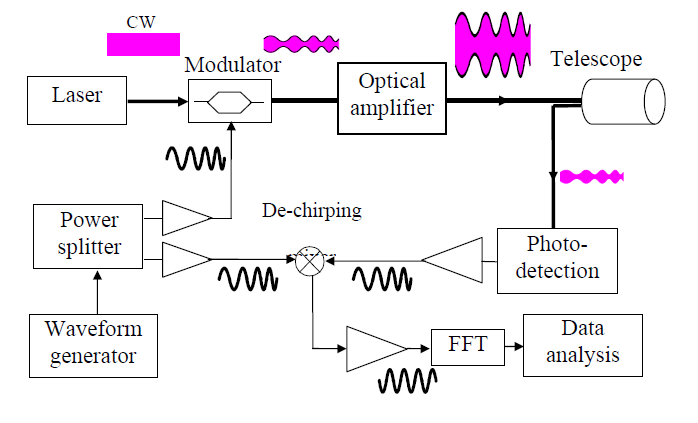
\includegraphics[width=0.8\columnwidth]{figs/direct}
	\vspace{1em}
	\caption{Direct detection architecture}
	\label{fig:directBlock}
\end{figure}

\subsection{Coherent Heterodyne Detection Architecture}
In coherent heterodyne detection the laser is split into two signals. One of these signals is modulated by the 
chirp waveform sent through an optical amplifier and out of the telescope. The other part of the the laser beam 
is used as the optical local oscillator. This LO signal is then shifted by an acousto-optic modulator to serve as
the intermediate frequency (IF) for coherent heterodyne detection. The IF is optically mixed with the returning 
signal from the telescope, the output of the optical mixer is fed into a balanced photodiode. The photodiode 
rejects the direct detection component. The output of the photodiode is filtered to isolate the heterdyne IF 
signal which is detected by an envelope detector. The IF signal is then mixed with the modulation waveform 
for dechirping. An FFT is then performed on the dechirped signal to recover the beat frequency.  

Optically mixing the returned signal with the LO helps mitigate the thermal noise in the photodiode. But because
the strong optical LO, the SNR is limited by the shot noise. The theoretical best SNR for a coherent heterodyne 
lidar is

\begin{equation}
\label{eq:heteroSNR}
SNR_{het}\approx\frac{\Re P_{sig}}{2qB_e}. 
\end{equation}

In this equation q is the electron charge. In coherent heterodyne detection the SNR is linearly proportional to 
the optical power, making it more suitable for low power operation. The most significant disadvantage of coherent
heterodyne detection is its complexity. The IF must be set much higher than the baseband, often in the GHz. This 
necessitates high speed optical detection and radio frequency (RF) processing circuitry. The IF envelope detection
process mixes the signal with RF noise which can further limit the SNR. Because of this the theoretical SNR defined
in eq \ref{eq:heteroSNR} has not been obtained in a coherent heterodyne implementation \cite{1319mmPerf}.  

\begin{figure}[H]
	\centering
	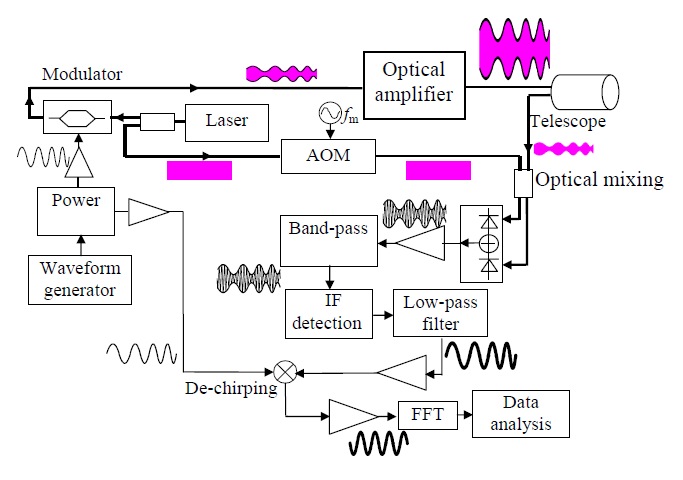
\includegraphics[width=0.8\columnwidth]{figs/heterodyne}
	\vspace{1em}
	\caption{Coherent heterodyne detection architecture}
	\label{fig:heterodyneBlock}
\end{figure}


\subsection{Homodyne Self-Chirped Detection Architecture}
\label{sec:homodyneSelf}
The homodyne self-chirped architecture was developed to maintain the receiver sensitivity obtained from coherent
heterodyne detection while minimizing complexity. In this simplified homodyne detection scheme the laser is 
modulated by the chirp waveform then split in two. One part of the modulated laser is amplified and sent out the
telescope, the other is used as the LO. The returned laser signal is mixed with the LO via a 2x2 optical coupler
the output of which is fed into a balanced photodetector. Because the LO is modulated with the same waveform as 
the transmitted laser, the optical mixing performs both optical detection and RF de-chirping. This reduces the 
amount of RF noise which is introduced to the detection signal. Performing an FFT on the output of the photodetector
yields the beat frequency. 

The simplification of the signal path in the homodyne self-chirped architecture results in a practical SNR closer
to the theoretical SNR in eq \ref{eq:heteroSNR} than the practical SNR of the coherent heterodyne architecture. 

\begin{figure}[H]
	\centering
	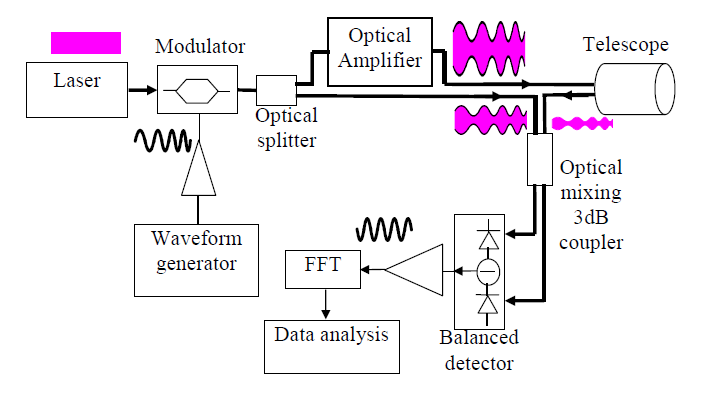
\includegraphics[width=0.8\columnwidth]{figs/simpleHomodyne}
	\vspace{1em}
	\caption{Homodyne self-chirped detection architecture}
	\label{fig:homodyneBlock}
\end{figure}

This architecture is popular for its performance and simplicity. Because it is being used by NASA for planetary 
landing missions \cite{amz12,amz12fiber,amz12p2,amz16coherent,pierrottet2009flight,pierrottet2011navigation}, it
has been selected as the basis for the simulation being reported on in this thesis. 



